\documentclass[a4paper,12pt]{article}
\usepackage[fleqn]{amsmath}
\usepackage{amssymb}
\usepackage{enumitem}
\usepackage{graphicx}
\graphicspath{ {./assets/} }

\newlist{list1}{itemize}{1}
\setlist[list1]{label=$\rightarrow$}

\newlist{list2}{itemize}{1}
\setlist[list2]{label=$\rightsquigarrow$}

\newlist{listHook}{itemize}{1}
\setlist[listHook]{label=$\hookrightarrow$}

\usepackage{mathtools}

\DeclarePairedDelimiter\abs{\lvert}{\rvert}%
\DeclarePairedDelimiter\norm{\lVert}{\rVert}%

\makeatletter
\let\oldabs\abs
\def\abs{\@ifstar{\oldabs}{\oldabs*}}

\let\oldnorm\norm
\def\norm{\@ifstar{\oldnorm}{\oldnorm*}}
\makeatother

\newcommand*{\Value}{\frac{1}{2}x^2}%

\begin{document}

\title{Physics Beyond}	
\author{Edward Jex}
\maketitle
\section*{Kinematics}
\subsection*{How to describe motion? (mathematically)}
\begin{list1}
	\item In maths we need a clear and precise definition.
	\item Motion is change in position over time.
	\begin{list2}
		\item What is space?
		\item What is time?
	\end{list2}
	\item How to describe motion?
	\begin{list2}
		\item Need a reference point / origin.
		\item Intuition about vectors.
		\begin{listHook}
			\item Rule of displacement from one point to another along a straight line
			\item Vector - from Latin "vehere" - to carry
		\end{listHook}
	\end{list2}
\end{list1}
To describe motion we need $f(t) \rightarrow x$ and $g(t) \rightarrow y$.
\begin{align*}
\vec{x}: \mathbb{R} & \rightarrow \text{Vector Space} \\
t & \mapsto \vec{x}(t) \\
\end{align*} 
\subsection*{What is vector space?}
\begin{list1}
	\item Euclidean 3-dimensional space. 
	\item For example, vector space of a 3 tuple of reals can be written as $\mathbb{R}^3$
	\item 
We say $V$ is a vector space if:
\begin{enumerate}
	\item $\mathbb{R} \cdot V \rightarrow V$
	\item Addition is commutative, associative, and has neutral element $\vec{O}$
	\item $(\lambda + \mu) \vec{v} = \lambda \vec{v} + \mu \vec{v} \hspace{2cm} \lambda, \mu \in \mathbb{R} \hspace{1cm} \vec{v} \in V$
	\item $(\lambda \mu)\vec{v} = \lambda(\mu \vec{v})$
	\item $1 \cdot \vec{v} = \vec{v}$
\end{enumerate}
\item We need to introduce a coordinate system.
\begin{align*}
\text{In 2 dimensions} \\
\vec{e}_1 & = \begin{bmatrix} 1 \\ 0 \end{bmatrix} \\
\vec{e}_2 & = \begin{bmatrix} 0 \\ 1 \end{bmatrix} \\
\text{In n dimensions} \\
\vec{e}_i & = \begin{bmatrix} 0 \\ 0 \\ \vdots \\ 1 \\ \vdots \\ 0 \\  \end{bmatrix} \\
\text{Where 1 is at index } i \\
\end{align*}
\item We can describe using unitary vectors:
\begin{align*}
\text{Two sets } & A, B \hspace{1cm} A \times B \hspace{0.5cm} \{(a,b)\;|\;a \in A, b \in B \} \\
& A \times A = A^2 \text{ Where } \times \text{ is the cartesian product}
\end{align*}
\end{list1}
\subsection*{What is happening mathematically?}
We have constructed a mapping $V \rightarrow \mathbb{R}^2$; it is $1 \rightarrow 1$\\
$\therefore$ For any vector, a pair of reals visa versa. 
\begin{align*}
\vec{x} \mapsto (x_1, x_2) \hspace{1cm} s.t \hspace{1cm} \vec{x} = x_1e_1 + x_2e_2
\end{align*}
\begin{enumerate}
	\item Note that for a basis, $e_1, e_2$ this mapping is one to one and onto (bijection) \\
		$\vec{x}(f) = (ae_1, be_2)$ $\leftarrow$ Linear combination of $e_1$ and $e_2$
	\item This means that we have an inverse mapping.
		\begin{align*}
			\mathbb{R} & \rightarrow E \\
			\begin{bmatrix} \lambda \\ \mu \\ \end{bmatrix} & \mapsto \lambda e_1 + \mu e_2 \\
		\end{align*}
		Coordinate systems translate $\mathbb{R}^2$ to vector E
	\item This mapping depends on the chosen coordinate system.
	\begin{list1}
		\item Coordinate system: (origin, two basis vectors)
		\begin{listHook}
			\item $(\vec{o}, \vec{e}_1, \vec{e}_2)$
			\item $\vec{e}_1, \vec{e}_1$ are linearly independent.
			\item We assume $\vec{e}_1 \perp \vec{e}_1$ $\rightarrow$ Is orthogonal (meet at 90 deg / $\frac{\pi}{2}$)
		\end{listHook}
	\end{list1}
\end{enumerate}
We have an improvement of our description:
\begin{align*}
\vec{x}: \mathbb{R} & \rightarrow \mathbb{R} \\
t & \mapsto \vec{x}(t) \hspace{2cm} \vec{x}(t) = \begin{bmatrix} x_1(t) \\ x_2(t) \\ \end{bmatrix} \hspace{2cm} x_1, x_2: \mathbb{R} \rightarrow \mathbb{R}
\end{align*}
\subsection*{Operators}
\begin{align*}
+: \> \mathbb{R}^n, \mathbb{R}^n & \rightarrow \mathbb{R}^n \\
(\begin{bmatrix} x_1 \\ \vdots \\ x_n \end{bmatrix}, \begin{bmatrix} y_1 \\ \vdots \\ y_n \end{bmatrix}) & \mapsto \begin{bmatrix} x_1 + y_1 \\ \vdots \\ x_n + y_n \end{bmatrix} \\\\
\cdot: \> \mathbb{R}, \mathbb{R}^n & \rightarrow \mathbb{R}^n \\
(\lambda, \begin{bmatrix} x_1 \\ \vdots \\ x_n \end{bmatrix}) & \mapsto \begin{bmatrix} \lambda x_1 \\ \vdots \\ \lambda x_n \end{bmatrix} \\\\
\mathbb{R}^x & = \{f: x \rightarrow \mathbb{R}\} \hspace{1cm} \text{Where $x$ is any set and f is a function}
\end{align*}
\section*{Maths foundations}
Current foundation: Set theory. What does that mean?
\begin{list1}
	\item Everything must be related back to sets.
	\item Relatively modern idea (2nd half of 20th century)
\end{list1}
\subsection*{Examples}
\begin{enumerate}
	\item Numbers:
	\begin{align*}
	0 & = \emptyset \text{ - empty set} \\
	1 & = \{\emptyset\} \text{ - set of the empty set} \\
	2 & = \{\emptyset, \{ \emptyset \}\} \text{ - set of the empty set and a set of the empty set} \\
	& \vdots 
	\end{align*}
	This means that natural numbers can be modelled using set theory. 
	\begin{list1}
		\item Model ideas = helps us to understand abstract ideas.
	\end{list1}
	\item Ordered pair: $(x, y)$ - order matters \\
	How can we model this using sets? (sets are unordered) \\
	$\{x,y\}$ doesn't work as unordered. \\
	$\{x, \{x,y\}\}$ could work for example. \\
	\item Relation \\
	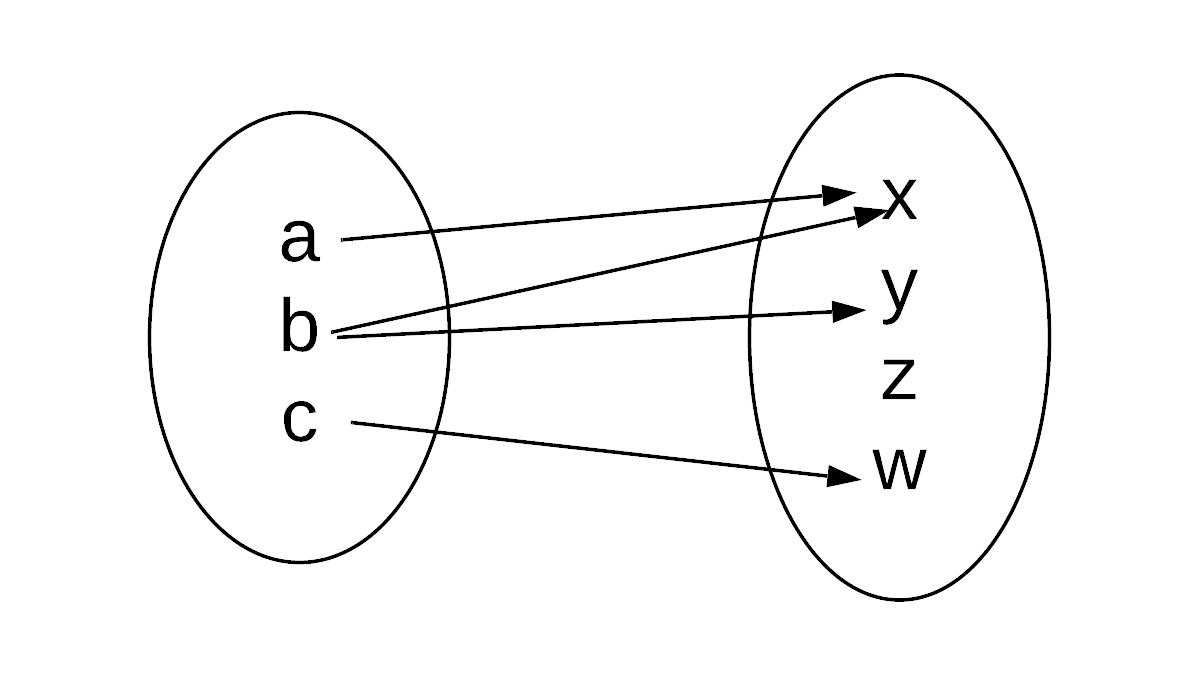
\includegraphics[scale=0.15]{fig1} \\
	Relation $\mathbb{R} \subseteq A \times B \\ ( A \times B = \{(a,b)\;|\; a \in A, b \in B \}$ \\
	Example 1:
	\begin{align*}
		x & \leqslant y \in \mathbb{R} \\
		& \leqslant \subseteq \mathbb{R} \times \mathbb{R} \\
		& (x,y) \in \leqslant
	\end{align*}
	Example 2 - Equivalence relation: \\
	(Example of vectors) \\
	\underline{Vectors:} \\
	\begin{enumerate}
		\item Idea: Rule of displacement of things along a straight line by a certain length (physics)
		\item Representation: Directed line segment
	\end{enumerate}
	How to model a vector? \\ 
	Consider the set L of all line segments in the plane \\
	\begin{list1}
		\item Subdivide L into disjointed subsets $[\vec{AB}]$ of line segments parallel, of same length and same orientation as $\vec{AB}$ \\
		$\vec{v} = [\vec{AB}]$ is a (model of a) vector. 
		\item Define a relation $\sim \subseteq L \times L$ ($\sim$ means equivalent to) \\
		\begin{align*}
			\vec{AB} \sim \vec{CD} : & \iff \text{They represent the same vector} \\
			& \iff [\vec{AB}] = [\vec{CD}] \\
			& \iff \vec{AB} \parallel \vec{CD},\;\norm{\vec{AB}} = \norm{\vec{CD}}
		\end{align*}
		In general, these three properties define what is called an equivalence relation.
	\end{list1}
	\item Functions / maps / mapping \\
	$ \rho: A \rightarrow B \hspace{1cm} x \mapsto f(x) $ \\
	Functions can be considered a type of relation. A relation is called a function if it is right-unique and left-total.
	\begin{align*}
		(x,y) \land (x,z) \Rightarrow & y = z \\
		& vx \in A \\
		& \exists y \in B \\
		& (x,y) \in f \\
		& y = f(x)
	\end{align*}
	Example: 
	\begin{align*}
		& \rho: \mathbb{R} \rightarrow \mathbb{R \hspace{1cm}} & x \mapsto x^2 \\ 
		& \rho \subseteq \mathbb{R} \times \mathbb{R} \hspace{1cm} 
		& \rho = \{ (x,y) \in \mathbb{R}^2 \;|\; y = x^2 \} \\
	\end{align*}
	The relation is the graph of the function.
\end{enumerate}
\section*{Motion}
Two areas:
\begin{itemize}
	\item Kinematics (mathematical modelling) 
	\item Dynamics (what causes motion)
\end{itemize}
\underline{Def}: Motion in the change in position in time. \\
position $\rightarrow$ space \hspace{2cm} time $\rightarrow$ time \\
$\rightsquigarrow$ Space + time too abstract $\rightarrow$ need to simplify \\
Space $\mapsto$ Euclidean geometry \\
Time $\mapsto$ Use $\mathbb{R}$ (Time is just a parameter) \\
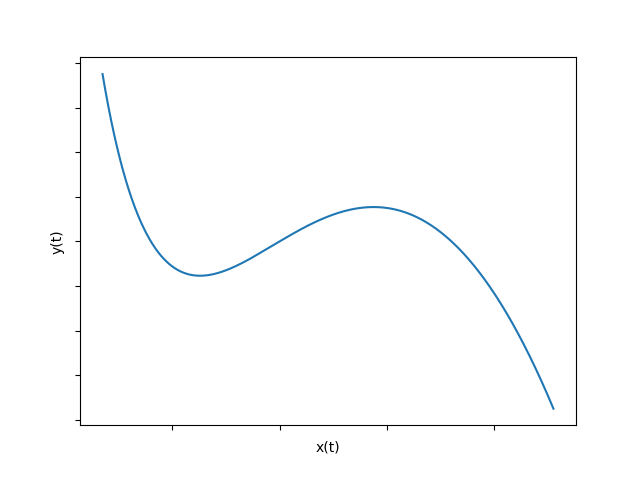
\includegraphics[scale=0.4]{example_curve} \\
Say this is the graph of $p(t)$ \\
$p: \mathbb{R} \rightarrow$ Space \\
$\rightsquigarrow$ Vectors + coordinates (reference frame) \\
\begin{align*}
	x: & \mathbb{R} \rightarrow \mathbb{R}^3 \\
	\vec{x} & = x_1e_1 + x_2e_2 + x_3e_3 \\
	\vec{x} & = \begin{bmatrix} x_1 \\ x_2 \\ x_3 \end{bmatrix}
\end{align*}
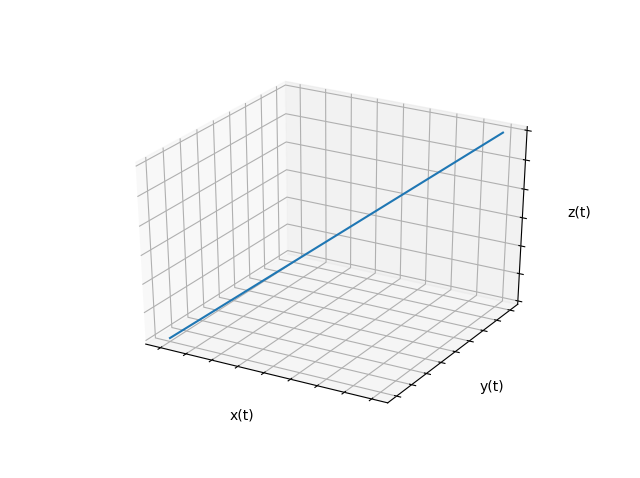
\includegraphics[scale=0.4]{fig2} \\
$\rightsquigarrow$ Algebra of geometric vectors translates directly into algebra of tuples.
\begin{align*}
	\vec{x} + \vec{y} & \longleftrightarrow 
	\begin{bmatrix} x_1 \\ x_2 \\ x_3 \end{bmatrix} +
	\begin{bmatrix} y_1 \\ y_2 \\ y_3 \end{bmatrix} =
	\begin{bmatrix} x_1 + y_1 \\ x_2 + y_2 \\ x_3 + y_3 \end{bmatrix} \\
	\lambda \vec{x} & \longleftrightarrow \lambda \begin{bmatrix} x_1 \\ x_2 \\ x_3 \end{bmatrix} =
	\begin{bmatrix} \lambda x_1 \\ \lambda x_2 \\ \lambda x_3 \end{bmatrix} \\
\end{align*}
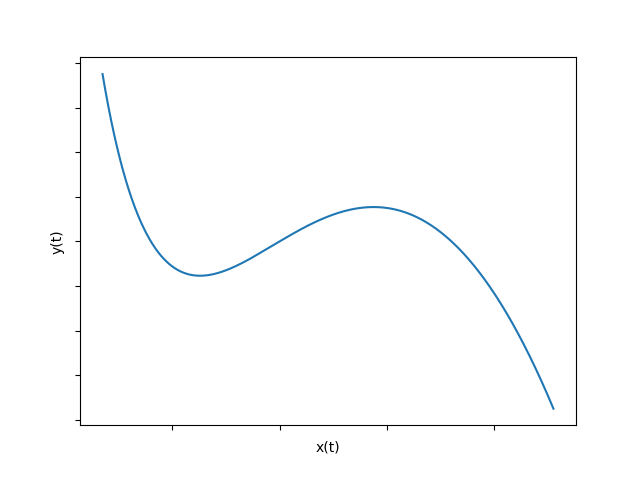
\includegraphics[scale=0.4]{example_curve} \\
\begin{align*}
	\vec{x}: & \mathbb{R} \rightarrow \mathbb{R}^3 \\
	t &\mapsto \vec{x}(t) \\\\
	\vec{x}(t) & = \begin{bmatrix} x_1(t) \\ x_2(t) \\ x_3(t) \end{bmatrix}
\end{align*}
\subsection*{Exaples}
\begin{enumerate}
	\item Motion along a line (with constant velocity)
	\begin{align*}
		\vec{x}(t)& = \vec{x_0} + t \vec{v} \\
		\begin{bmatrix} x_1(t) \\ x_2(t) \\ x_3(t) \end{bmatrix} & = 
		\begin{bmatrix} x_{01} \\ x_{02} \\ x_{03} \end{bmatrix} +
		t \begin{bmatrix} v_1 \\ v_2 \\ v_3 \end{bmatrix} \\	
		& = \begin{bmatrix} x_{01} + t v_1\\ x_{02} + t v_2 \\ x_{03} + t v_3 \end{bmatrix}
	\end{align*}
	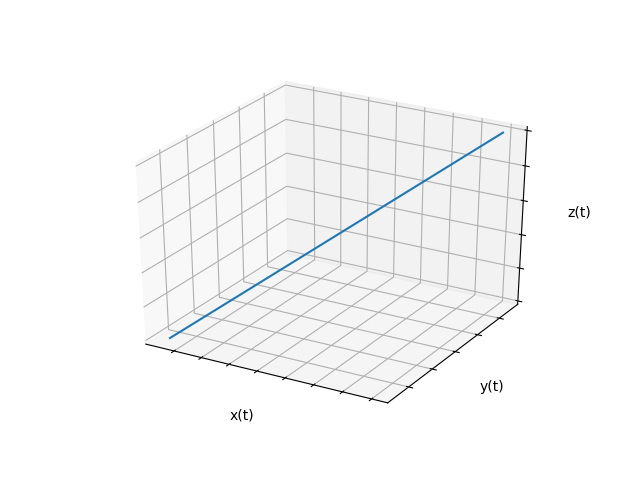
\includegraphics[scale=0.4]{straigt_line}
	\item Circular motion \\
	$\vec{x}(t) = r \begin{bmatrix} \cos(\rho t) \\ \sin(\rho t) \end{bmatrix}$ \\
	Where $\rho$ some function and $r$ is the radius.\\
	If it is uniform: \\
	\begin{align*}
		\vec{x}(t) & = r \begin{bmatrix} \cos(\omega t) \\ \sin(\omega t) \end{bmatrix} \\
		\omega & \in \mathbb{R} | \{0\} \hspace{2cm} \omega = \frac{2\pi}{T}
	\end{align*}
	Where $T$ is the time period.\\
	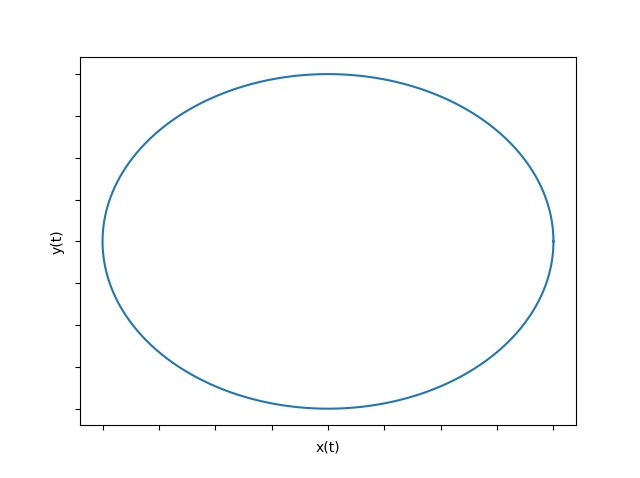
\includegraphics[scale=0.4]{circle} \\
	\item Uniform spiral
	It is just like a circle, but with linear motion in the z-axis.
	\begin{align*}
		\vec{x}(f) = \begin{bmatrix} r \cos \omega t \\ r \sin \omega t \\ v t \end{bmatrix}
	\end{align*}
	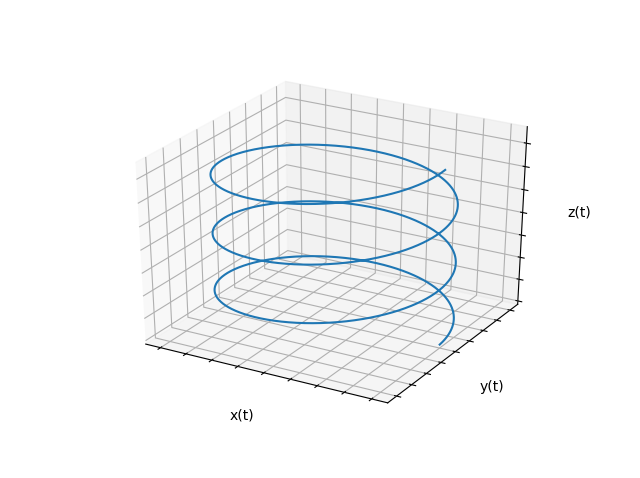
\includegraphics[scale=0.4]{spiral}
\end{enumerate}
\section*{Kinematics - reminder}
\begin{list2}
	\item Done with modelling motion mathematically? \\ $\hookrightarrow$ How to study the physics of motion?
	\item What is the natural state of motion? \\ - Without physical interaction. 
	\item At rest? (Aristotle) $\times$
	\item Uniform motion (Newton) \\ $\hookrightarrow$ Why?
	\begin{listHook}
		\item Changing reference frame to a moving one $\rightarrow$ object at rest relativity. 
		\item But we cannot answer/ decide what the natural state of motion is in this stage.
	\end{listHook}
\end{list2}
\underline{Observation}: State of motion changes due to physical interaction $\rightarrow$ Lets model physical interaction with forces. 
What is the change in motion due to force?
\begin{list2}
	\item The shape of the trajectory is curved 
	\item We don't know how to model that! \\ $\hookrightarrow$ Back to maths
\end{list2}
\section*{Kinematics 2}
\subsection*{Modelling change in motion}
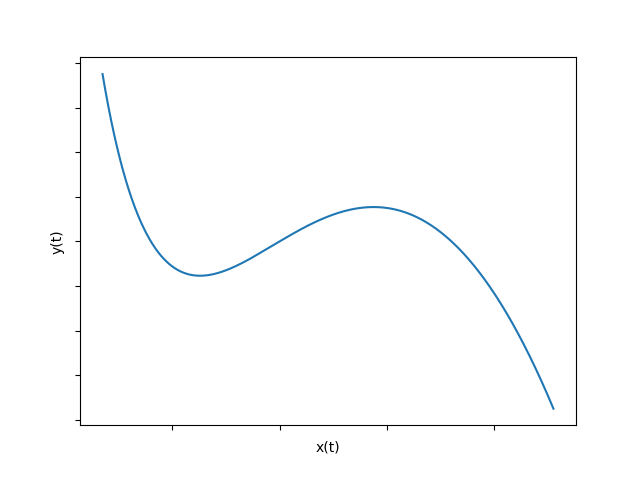
\includegraphics[scale=0.4]{example_curve} \\
Take two points on the above curve, $\vec{x}(t_0)$ and $\vec{x}(t)$.
The change of displacement is $\Delta \vec{x}$. We know that velocity is change in displacement over change in time so we can find that using:
\begin{align*}
\vec{v} & = \frac{\Delta \vec{x}}{\Delta t} \\
& = \frac{\vec{x}(t)-\vec{t_0}}{t-t_0}
\end{align*}
This gives us the average velocity between $t_0$ and $t$. We need to be able to find the velocity at every point in time $t_0$
\begin{align*}
\vec{v}: \mathbb{R} & \rightarrow \mathbb{R}^3 \\
t & \mapsto \text{velocity at t}
\end{align*}
Problem: We need a second time $t = t_0 + h$ for $\vec{v}(t_0)$, but there is no natural choice for h.
We notice for more precision we need to make h as small as possible!
\begin{align*}
&\lim_{h \to 0} \frac{\vec{x}(t+h)-\vec{x}(t)}{h} \\
= & \frac{d\vec{x}}{dt} \text{ Leibniz notation} \\
= & \dot{\vec{x}}(t) \text{ Newton notation}\\
\end{align*}
Differentiation on vectors is just element wise:
\begin{align*}
\frac{d}{dt} \begin{bmatrix} R \cos \omega t \\ R \sin \omega t \end{bmatrix} = \omega R \begin{bmatrix}
-\sin \omega t \\ \cos \omega t \end{bmatrix}
\end{align*}
Limits create paradoxes:
Take $\lim_{h \to 0} \frac{\vec{x}(t+h)-\vec{x}(t)}{h}$. This works mathematically but causes a conceptual problem: How can something change at one point in time? \\
$\rightsquigarrow$ Solution: Use infinitesimals \\ 
$\rightarrow$ Numbers that are not provably not 0. 
Idea: If we zoom in on any curve enough, begins to look like a straight line: e.g. Earth looks flat. \\
How can we model this mathematically? \\
$\rightsquigarrow$ Around each point $\vec{x}(t_0)$ the curve is made up of infinitesimal line segments. \\
Geometrically: A tangent at $\vec{x}(t_0)$ touches the curve at $\vec{x}(t_0)$ \\ 
$\hookrightarrow$ We take this to mean that it intersects with the curve at an infinitesimal line segment \\
$\hookrightarrow$ Infinitesimal line segment is the intersection of the tangent and the curve. \\
Problem: Do not have a rigorous definition of a tangent at a curve! \\
$\rightarrow$ But we know: Every line that intersects the circle in one points is a tangent $\rightsquigarrow$ Use that!
\\ 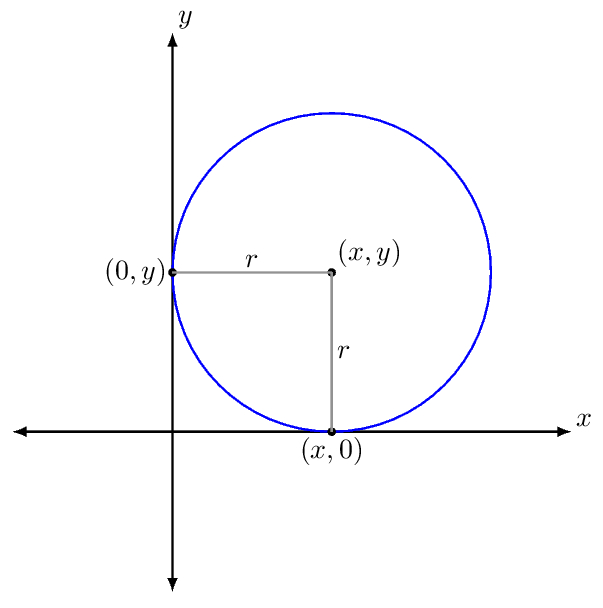
\includegraphics[scale=0.4]{circle_tangent} \\
Take the radius, r, to be 1 and the center to be $(0,1)$.
\begin{align*}
&\text{Eqation of circle:} \\
& c: (x-0)^2 + (y-1)^2 = 1 \\
&\text{If we take our tangent, t to be the y axis:} \\
& t: y = 0 \\
&\text{Sub into c:} \\
& x^2 +1 = 1 \\
& \Rightarrow x^2 = 0 \\
& \therefore c \cap t = \{(d,0)\;|\;d^2=0\} \\ 
\end{align*}
$\rightsquigarrow$ Define first order infinitesimals as $D = \{d \in R\;|\;d^2=0\}$ where $R = \mathbb{R} \cup \{\text{infinitesimal numbers}\}$
Are such infinitesimals going to solve problems?
\begin{align*}
f(x) & = x^2 \\
\Rightarrow & f(x + d) \hspace{2cm} d \in D \\
& = ( x + d )^2 \\
& = x^2 + 2dx + d^2 \\
& = x^2 + 2dx \\
& = f(x) + f'(x) \cdot d \\\\
f(x) & = x^3 \\
\Rightarrow & f(x + d) \\
& = (x + d)^3 \\
& = x^3 + 3x^2d + 3xd^2 + d^3 \\
& = x^3 + 3x^2d \\
& = f(x) + f'(x) \cdot d \\
\end{align*}
\end{document}